\documentclass[default,compress]{beamer}

\usepackage[utf8]{inputenc}
\usepackage{beamerthemesplit}
\usepackage{amsmath}
\usepackage{amssymb}
\usepackage{graphicx}
\usepackage{textpos}
\usepackage{multicol}
\usepackage{minted}

\hypersetup{colorlinks=true, urlcolor=black}

\mode<presentation>

\setbeamertemplate{navigation symbols}{}

\title{The PlasmaPy Project: Toward an Open Source Software Ecosystem for Plasma Physics}

\author{
    The PlasmaPy Community:
    N.\ A.\ Murphy,\textsuperscript{1}
    D.\ Sta\'nczak,\textsuperscript{2}
    E.~T.~Everson,\textsuperscript{3} 
    P.\ M.\ Kozlowski,\textsuperscript{4}
    R.\ Malhotra,\textsuperscript{5}
    S.\ J.\ Langendorf,\textsuperscript{4}
    A.\ J.\ Leonard,\textsuperscript{6}
    D.\ Stansby,\textsuperscript{7}
    S.\ J.\ Mumford,\textsuperscript{8}
    J.~P.\ Beckers,\textsuperscript{9}
    T.\ N.\ Parashar,\textsuperscript{10}
    D.\ Schaffner,\textsuperscript{12} \&
    S.\ T.\ Vincena \textsuperscript{3}
}

\institute{
    \textsuperscript{1}Center for Astrophysics $\vert$ Harvard \& Smithsonian,
    \textsuperscript{2}University of Warsaw,
    \textsuperscript{3}UCLA,
    \textsuperscript{4}LANL,
    \textsuperscript{5}Chandigarh University,
    \textsuperscript{6}Aperio Software, 
    \textsuperscript{7}Imperial College London,
    \textsuperscript{8}University of Sheffield,
    \textsuperscript{9}ASML
    \textsuperscript{10}University of Delaware,\\
    \textsuperscript{11}Bryn Mawr College
}

\date{\footnotesize{
    61th Annual Meeting of the APS Division of Plasma Physics\\
    Ft.\ Lauderdale, Florida, USA,
    October 21--25, 2019
}}

\begin{document}


\begin{frame}[plain]

    \titlepage
    
    \begin{center}
        \href{https://doi.org/10.5281/zenodo.3491170}{
\includegraphics[height=0.47cm]{DPP_2019_DOI.png}}
    \end{center}
 
    \begin{textblock}{1}(-0.9,-1.43)
      \href{http://www.plasmapy.org/}{
\includegraphics[height=0.57cm]{plasmapy-logo.png}}
    \end{textblock}
        
    \begin{textblock}{1}(12.4,-1.43)
      \href{https://creativecommons.org/licenses/by/4.0/}{
\includegraphics[height=0.57cm]{by.png}}
    \end{textblock}
    
\end{frame}


\begin{frame}[plain]
    \frametitle{Introduction}
    \begin{itemize}
    \item In recent years, researchers in several different subfields of physics and astronomy have collaboratively developed core Python packages such as \href{http://www.astropy.org/}{Astropy}\footnote{\href{https://arxiv.org/abs/1801.02634}{Astropy Collaboration (2018)}} and \href{http://sunpy.org/}{SunPy}\footnote{\href{https://doi.org/10.1088/1749-4699/8/1/014009}{SunPy Community (2015)}} 
    \item These packages provide core functionality and common frameworks for data analysis and visualization
    \item A similar open source package for plasma physics would greatly benefit our field
    \item \textbf{We are developing \href{http://www.plasmapy.org/}{PlasmaPy}: a community-developed and community-driven open source core Python package for plasma physics}
    \end{itemize}
\end{frame}


\begin{frame}[plain]
    \frametitle{The goal of PlasmaPy is to facilitate a fully open source software ecosystem for plasma physics}
    \begin{center}
        \href{
            https://github.com/PlasmaPy/plasmapy
        }{
            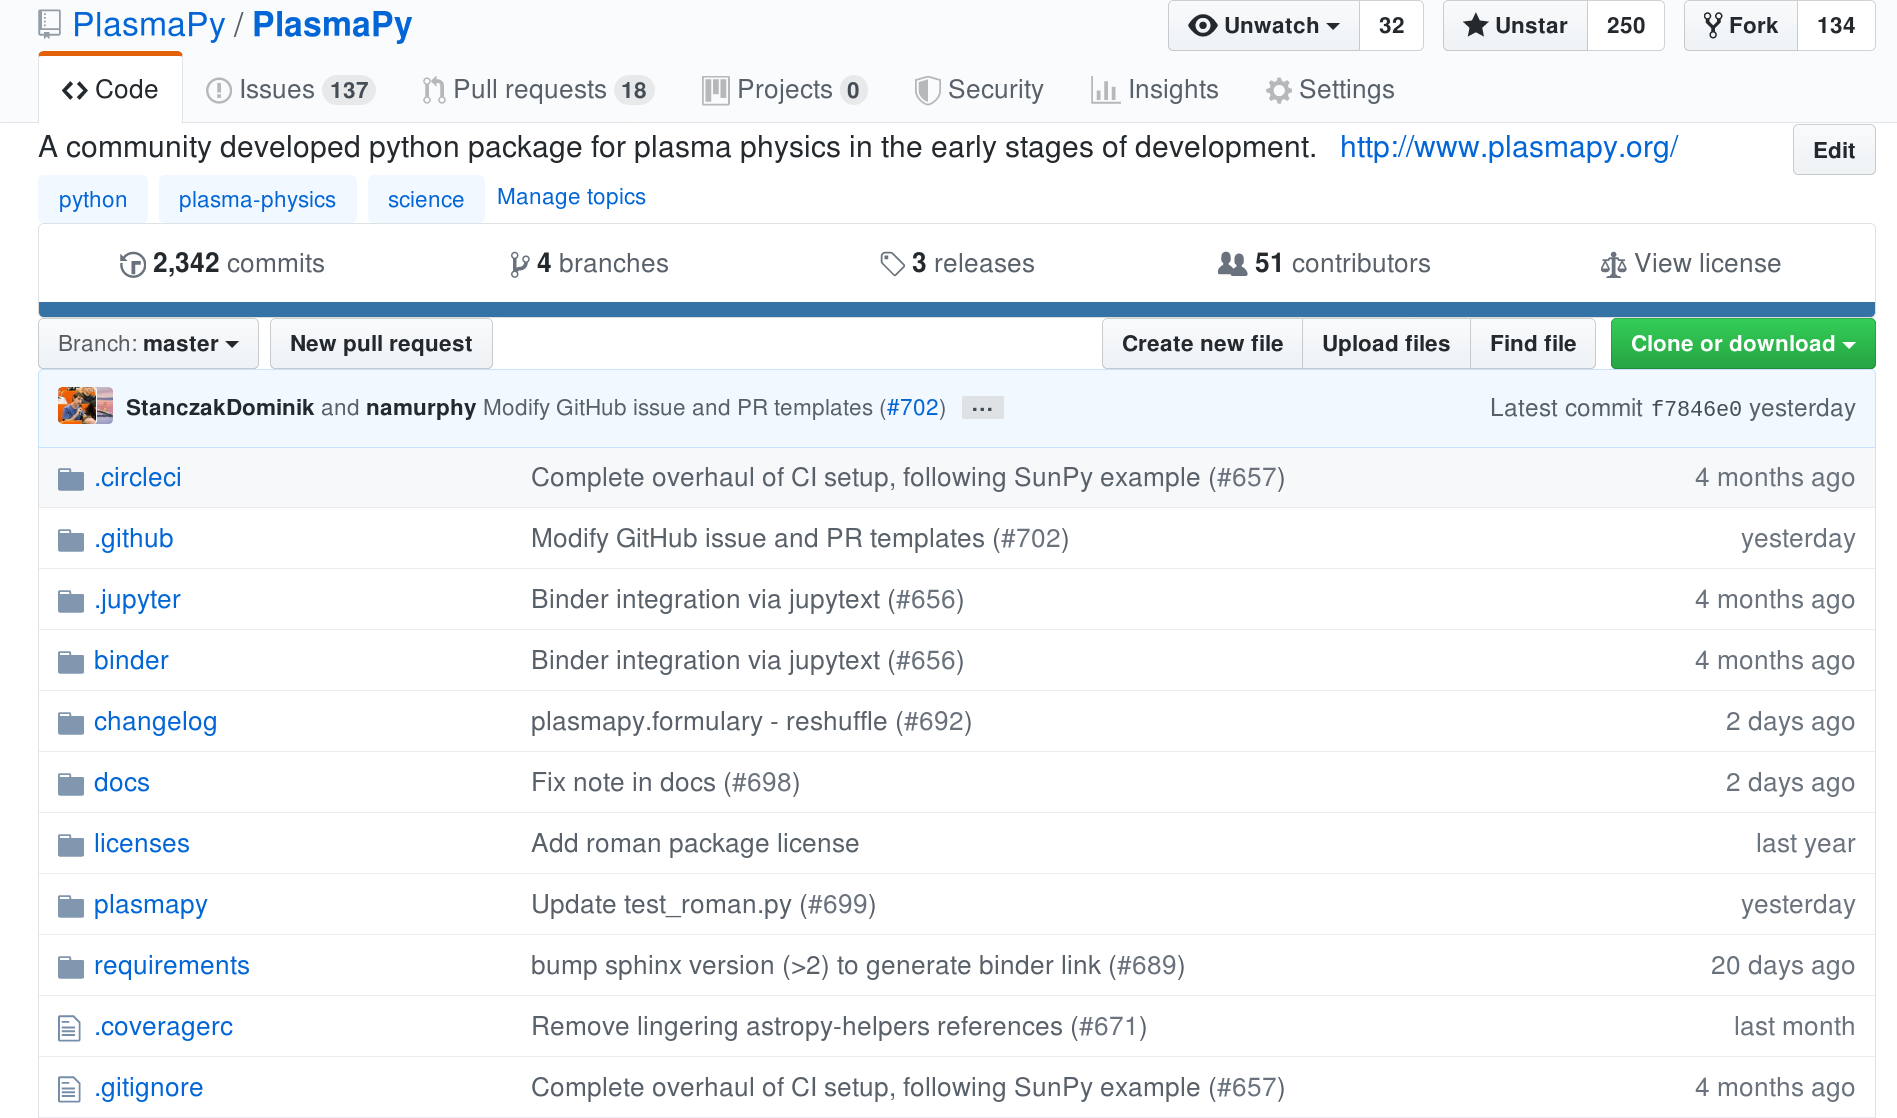
\includegraphics[width=11.0cm]{PlasmaPy_mainpage.png}
        }
    \end{center}
\end{frame}


\begin{frame}[plain]
    \frametitle{We have a ``roll your own'' culture for code development}
    \begin{itemize}
    \item We tend to be self-taught as programmers
    \item Time pressure prevents us from improving programming skills
    \item Software is often written ``in-house'' as needed
    \item Code is often written in a rush to get a paper out
    \item Code is often written for a specific purpose, which makes it hard to generalize
    \item Documentation is often insufficient
    \item Codes often lack a testing framework
    \item Frequent duplication of functionality between groups
    \item Packages lack interoperability
    \end{itemize}
\end{frame}


\begin{frame}[plain]
    \frametitle{Consequences of ``roll your own'' culture}
    \begin{itemize}
    \item \textbf{Beginning research is difficult} due to software overhead
    \item \textbf{Collaboration is difficult} due to lack of interoperability
    \item Plasma research is much \textbf{less reproducible}
    \item Research can be \textbf{frustrating}
    \end{itemize}
        \vspace{3mm}
    \begin{center}
        \fbox{\parbox{100mm}{\Large{
            Plasma science can learn from what other fields are doing to change ``roll your own'' culture.
            }
        }}
    \end{center}
\end{frame}


\begin{frame}[plain]
    \frametitle{PlasmaPy uses Astropy's open development model}
    \begin{itemize}
    \item Release code under an \textbf{open source license}
    \item \textbf{Develop openly} on GitHub
    \item \textbf{Anyone may contribute} 
    \item New contributors are \textbf{actively welcomed}
    \item Adopt a \textbf{code of conduct}
    \end{itemize}
\end{frame}


\begin{frame}[plain]
    \frametitle{Planned subpackages for PlasmaPy version 0.3.0}  
    \begin{itemize}
    \item \mintinline{python}{atomic} provides access to basic atomic data
    \item \mintinline{python}{classes} contains prototype base classes
    \item \mintinline{python}{diagnostics} will provide experimental analysis tools
    \item \mintinline{python}{formulary} contains plasma parameters, transport coefficients, and mathematical functions
    \item \mintinline{python}{simulation} contains a particle pusher and will contain broader simulation capabilities
    \item \mintinline{python}{utils} provides utilities used throughout the package
    \end{itemize}
\end{frame}


\defverbatim[colored]\AstropyUnits{\vspace{-2mm}
    \begin{minted}[fontsize=\normalsize,
                   framesep=3mm,
                   autogobble,
                   ]{pycon}
    >>> from astropy import units
    
    >>> distance = 44 * units.imperial.mile
    >>> time = 30 * units.minute
    >>> distance / time
    <Quantity 88.0 mi / h>

    >>> (1.21 * units.GW).cgs
    <Quantity 1.21e+16 erg / s>
    
    >>> 2 * units.m + 4 * units.m / units.s
    UnitConversionError: Can only apply 'add' function 
    to quantities with compatible dimensions
    \end{minted}
}


\begin{frame}[plain]
    \frametitle{PlasmaPy uses the \href{http://docs.astropy.org/en/stable/units/}{\mintinline[style=fruity]{python}{astropy.units}} package for units}
    This package creates \mintinline{python}{Quantity} objects with attached units.\\ 
    \AstropyUnits
\end{frame}


\defverbatim[colored]\atomic{
    \begin{minted}[fontsize=\normalsize,
                   framesep=3mm,
                   style=emacs,
                   autogobble
                   ]{pycon}
    >>> from plasmapy.atomic import Particle
    
    >>> alpha = Particle("He-4++")
    >>> alpha.mass
    <Quantity 6.64465709e-27 kg>
    
    >>> electron = Particle("e-")
    >>> electron.charge
    <Quantity -1.60217662e-19 C>
    >>> electron.is_category(require={"lepton", "fermion"})
    True
    >>> ~electron  # find antiparticle with invert operator
    Particle("e+")
    \end{minted}
}


\begin{frame}[plain]
    \frametitle{PlasmaPy's \mintinline{python}{atomic} subpackage provides functional and object-oriented interfaces to particle data}
    Instances of the \mintinline{python}{Particle} class may be used to represent individual atoms, ions, or elementary particles.
    \\ \vspace{-2mm}
    \atomic
\end{frame}


\defverbatim[colored]\physics{
    \begin{minted}[fontsize=\normalsize,
                   framesep=3mm,
                   style=emacs,
                   autogobble
                   ]{pycon}
    >>> from plasmapy.formulary import *
    
    >>> n_e = 1e15 * u.m ** -3
    >>> T_e = 6 * u.MK
    >>> B = 0.2 * u.T
    
    >>> Debye_length(n_e = n_e, T_e = T_e)
    <Quantity 0.00534541 m>
    
    >>> upper_hybrid_frequency(B, n_e)
    <Quantity 3.52216092e+10 rad / s>
    
    >>> n_i = 5e19 * u.m ** -3
    >>> inertial_length(n_i, 'D+')
    <Quantity 0.04553085 m>  
    \end{minted}
}


\begin{frame}[plain]
    \frametitle{The \mintinline{python}{formulary} subpackage provides functions to calculate plasma parameters}
    \physics
\end{frame}


\defverbatim[colored]\dielectric{
    \begin{minted}[fontsize=\small,
                   framesep=3mm,
                   style=emacs,
                   autogobble
                   ]{pycon}
    >>> B = 2 * u.T
    >>> species = ['e-', 'D+']
    >>> n = [1e18 * u.m ** -3, 1e18 * u.m ** -3]
    >>> omega = 3.7e9 * (2 * pi) * (u.rad / u.s)
    
    >>> L, R, P = cold_plasma_permittivity_LRP(B, species, n, omega)
    
    >>> L
    <Quantity 0.63333549>
    >>> R
    <Quantity 1.41512254>
    >>> P
    <Quantity -4.8903104>
    \end{minted}
}


\defverbatim[colored]\classicaltransport{
    \begin{minted}[fontsize=\small,
                   framesep=3mm,
                   style=emacs,
                   autogobble
                   ]{pycon}
    >>> T = 1 * u.MK
    >>> n = 5e15 * u.m ** -3
    >>> particles = ('e-', 'p+')
    >>> collision_frequency(T, n, particles)
    <Quantity 443.02775451 Hz>
    >>> coupling_parameter(T, n, particles)
    <Quantity 4.60608476e-06>

    >>> T_e, n_e = 0.6 * u.keV, 1e16 * u.cm ** -3
    >>> T_p, n_p = 0.8 * u.keV, 1e16 * u.cm ** -3
    >>> braginskii = ClassicalTransport(T_e, n_e, T_p, n_p, 'p+')
    >>> braginskii.ion_thermal_conductivity
    <Quantity 132961.01785222 W / (K m)>
    >>> braginskii.electron_viscosity
    <Quantity [0.02734206, 0.02733305, 0.02733305, 0., 0.] Pa s>

    \end{minted}
}


\begin{frame}[plain]
    \frametitle{\texttt{plasmapy.formulary} includes functions to calculate collision parameters and transport coefficients}
    \classicaltransport
\end{frame}


\begin{frame}[plain]
    \frametitle{
        \texttt{plasmapy.simulation} contains a particle pusher\footnote{
            More examples:\
            \href{
                http://docs.plasmapy.org/en/latest/auto_examples
                }{
                    \texttt{http://docs.plasmapy.org/en/latest/auto\_examples}
            }
        }
    }
    \begin{center}
        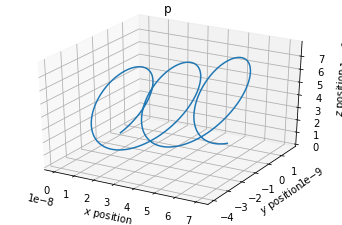
\includegraphics[width=9cm]{ExB_example.png}
    \end{center}
\end{frame}


\begin{frame}[plain]
    \frametitle{Code development priorities for 2020}
    \begin{itemize}
    \item \textbf{Refactor existing code and tests}
        \begin{itemize}
        \item Strengthen foundation for future development
        \end{itemize}
    \item \textbf{Dispersion relation solvers}
        \begin{itemize}
        \item Design of interface currently underway
        \end{itemize}
    \item \textbf{Plasma diagnostic analysis tools}
        \begin{itemize}
        \item Diagnostic classes that can be instantiated for a specific probe
        \item Initial focus on Swept Langmuir and Triple probes
        \item Provide various calculation methods for I$_{sat}$, T$_e$, n$_e$, and V$_p$ (all with associated statistics)
        \item Develop architecture for multi-trace data analysis
        \end{itemize}
    \item \textbf{Expand numerical simulation capabilities}
        \begin{itemize}
        \item Classes to represent problem setup independent of numerics
        \item Metadata schemas (akin to openPMD)
        \item Interchangeable simulation modules
        \end{itemize}
    \item \textbf{Educational Jupyter notebooks}
        \begin{itemize}
        \item Tutorials that introduce plasma concepts with PlasmaPy
        \end{itemize}
    \end{itemize}
\end{frame}


\begin{frame}[plain]
    \frametitle{Organizational infrastructure is needed for long-term software sustainability}
    \begin{itemize}
    \item The \textbf{Coordinating Committee} oversees the PlasmaPy project and code base
        \begin{itemize}
        \item Ideally have representation across plasma subdisciplines
        \item Currently strong representation by heliophysicists
        \end{itemize}
    \item In practice, \textbf{most coordination is done informally}
        \begin{itemize}
        \item GitHub issues and pull requests
        \item Matrix/Gitter channel for text-based chat
        \item Biweekly community meetings
        \end{itemize}
    \item \textbf{PlasmaPy Enhancement Proposals (PLEPs)} allow the community to influence the direction of PlasmaPy
    \item The \textbf{PlasmaPy Community on Zenodo}\footnote{
    \href{
        https://zenodo.org/communities/plasmapy
        }{
        https://zenodo.org/communities/plasmapy
        }
    } contains presentations, PLEPs, white papers, and proposals
    \end{itemize}
\end{frame}


\begin{frame}[plain]
    \frametitle{PlasmaPy has documentation!\footnote{https://docs.plasmapy.org}}
    \begin{itemize}
    \item Each function and class has a docstring
    \item Subpackages have narrative documentation
    \item Docstrings and narrative documentation are transformed into online documentation
    \item Test builds of documentation are run for every pull request
    \item Code examples are tested to make sure output is correct
    \end{itemize}
\end{frame}


\begin{frame}[plain]
    \frametitle{PlasmaPy has tests!}
    \begin{itemize}
    \item All pull requests undergo \textbf{continuous integration testing}
        \begin{itemize}
        \item We know right away when we break something
        \item Useful error messages help narrow down causes
        \end{itemize}
    \item Automated \textbf{test coverage checks} 
    show which lines of code are not covered by tests
        \begin{itemize}
        \item We know what tests we still need to write
        \item We can find and delete unused portions of code
        \end{itemize}
    \item Helpful practices
        \begin{itemize}
        \item Write tests before production code
        \item Turn bugs into tests cases
        \end{itemize}
    \end{itemize}
\end{frame}


\begin{frame}[plain]
    \frametitle{Anticipated benefits of PlasmaPy}
    \begin{itemize}
    \item More reproducible, open, and efficient research
    \item Reduce duplication of functionality
    \item Reduce barriers to entry for plasma research
    \item Let students hit the ground running on first research projects
    \item Help us learn collaborative code development practices
        \begin{itemize}
        \item Helpful for students entering industry upon graduation
        \end{itemize}
    \item Provide well-documented and well-tested software
    \item Improve interoperability between different packages
    \item Enable cross-disciplinary and cross-device studies
    \item Reduce software development overhead costs for experiments
    \item Create tools for plasma pedagogy
    \end{itemize}    
\end{frame}


\begin{frame}[plain]
    \frametitle{Summary}
    \begin{itemize}
    \item We are developing PlasmaPy to contain core functionality for an \textbf{open source software ecosystem} for plasma science
        \begin{itemize}
        \item Version 0.3.0 to be released early next year
        \end{itemize}
    \item PlasmaPy is building bridges among laboratory, heliospheric, and astrophysical plasma physicists
        \begin{itemize}
        \item Active in Python in Heliophysics Community
        \end{itemize}
    \item A new five-year, \$2.4M collaborative NSF CSSI award\footnote{Our proposal is available online at:
    N.\ A.\ Murphy, E.\ Everson, S.\ Vincena, T.\ Parashar, \& D.\ Schaffner (2019), Zenodo, doi:\ 
    \href{https://doi.org/10.5281/zenodo.3406803}{10.5281/zenodo.3406803}} will support ongoing development for fundamental plasma science
    \item If there is functionality that you would like in PlasmaPy, please \href{https://github.com/PlasmaPy/PlasmaPy/issues/new}{raise an issue} in our GitHub repository!
    \end{itemize}
\end{frame}


\begin{frame}[plain]
    \frametitle{We invite you to join the PlasmaPy community}
    \begin{itemize}
    \item Join conversation on Matrix channel
        \begin{center}
            \small{\texttt{https://riot.im/app/\#/room/\#plasmapy:openastronomy.org}}
        \end{center}
    \item Join PlasmaPy's email list
        \begin{center}
                \small{\texttt{https://groups.google.com/forum/\#!forum/plasmapy}}
        \end{center}
    \item Begin a discussion on Discourse
        \begin{center}
            \href{
                    https://plasmapy.discourse.group/
                }{
                \small{\texttt{https://plasmapy.discourse.group}}}
        \end{center}
    \item Submit feature requests via GitHub issues, or contribute code, documentation, tutorials, and examples at:
        \begin{center}
            \href{
                https://github.com/PlasmaPy/plasmapy
            }{
                \small{\texttt{https://github.com/PlasmaPy/plasmapy}}
            }
        \end{center}
    \item Organize community events
    \item Advocate for openness, reproducibility, equity, \& inclusion in plasma science
    \end{itemize}
\end{frame}

\end{document}


\begin{frame}[plain]
    \frametitle{Anticipated benefits of PlasmaPy}
    \begin{itemize}
    \item More reproducible, open, and efficient research
    \item Reduce duplication of functionality
    \item Reduce barriers to entry for plasma research
    \item Let students hit the ground running on first research projects
    \item Help plasma community learn collaborative code development practices
        \begin{itemize}
        \item Helpful for students entering industry upon graduation
        \end{itemize}
    \item Provide well-documented and well-tested software
    \item Improve interoperability between different packages
    \item Enable cross-disciplinary and cross-device studies
    \item Reduce software development overhead costs for experiments
    \item Create tools for plasma pedagogy
    \end{itemize}    
\end{frame}


\begin{frame}[plain]
    \frametitle{Sign-up sheet for PlasmaPy email list}
    \hspace{1.1mm}\textbf{Name} \hspace{37mm} \textbf{Email address}\vspace{4mm}\\
    \vspace{4mm}
    $\rule[-0.3mm]{48mm}{0.16mm}$\hspace{2mm}$\rule[-0.3mm]{56mm}{0.16mm}$\\
    \vspace{4mm}
    $\rule[-0.3mm]{48mm}{0.16mm}$\hspace{2mm}$\rule[-0.3mm]{56mm}{0.16mm}$\\
    \vspace{4mm}
    $\rule[-0.3mm]{48mm}{0.16mm}$\hspace{2mm}$\rule[-0.3mm]{56mm}{0.16mm}$\\
    \vspace{4mm}
    $\rule[-0.3mm]{48mm}{0.16mm}$\hspace{2mm}$\rule[-0.3mm]{56mm}{0.16mm}$\\
    \vspace{4mm}
    $\rule[-0.3mm]{48mm}{0.16mm}$\hspace{2mm}$\rule[-0.3mm]{56mm}{0.16mm}$\\
    \vspace{4mm}
    $\rule[-0.3mm]{48mm}{0.16mm}$\hspace{2mm}$\rule[-0.3mm]{56mm}{0.16mm}$\\
    \vspace{4mm}
    $\rule[-0.3mm]{48mm}{0.16mm}$\hspace{2mm}$\rule[-0.3mm]{56mm}{0.16mm}$\\
    \vspace{4mm}
    $\rule[-0.3mm]{48mm}{0.16mm}$\hspace{2mm}$\rule[-0.3mm]{56mm}{0.16mm}$\\
\end{frame}

